\documentclass[11pt,a4paper,twoside]{article}
\usepackage[margin=2cm]{geometry}
\usepackage[fleqn]{amsmath}
\usepackage{amsfonts}
\usepackage{amssymb}
\usepackage{mathtools}
\usepackage{makeidx}
\usepackage{tabularx}
\usepackage{multirow}
\usepackage{enumerate}
\usepackage[mathscr]{euscript}
\usepackage{framed}
\usepackage{physics}
\usepackage{siunitx}
\usepackage{upgreek}
\usepackage{chemmacros}
\usepackage{graphicx}
\usepackage[version=4]{mhchem}
\graphicspath{{.}{graphics}}



%%%%%%%%%%%%%%%%%%%% Maths %%%%%%%%%%%%%%%%%%%%%%%%

\numberwithin{equation}{section}
\setlength\mathindent{5mm}
\newcommand{\eqn}[1]{Eq.~\eqref{#1}}
\newcommand{\eqs}[2]{Eqs.~\eqref{#1} and~\eqref{#2}}
\newcommand{\DrG}{\ensuremath{\Delta_{\mathrm{r}}G}}
\newcommand{\DrH}{\ensuremath{\Delta_{\mathrm{r}}H}}
\newcommand{\std}{^{\standardstate}}
\newcommand{\ca}{\ensuremath{c_{\rm a}}}
\newcommand{\kn}[1]{$k$\textsubscript{$#1$}}
% Define a new column type for centered text with equal width
\newcolumntype{C}{>{\centering\arraybackslash}X}

%%%%%%%%%%%%%%%% Title %%%%%%%%%%%%%%%%%%%%%%%%%%%%%


\title{\bfseries%
Formula Sheet}
\author{
compiled by George Trenins}

\makeatletter
\def\maketitle{
    \begingroup
    \centering
    \bfseries
    \ifx\@title\@empty\else
        \LARGE \@title \par \vskip 5pt % Adjust the value as desired
    \fi
	\normalfont
    \ifx\@author\@empty\else
        \vskip 2pt % Adjust the value as desired
        \large \@author \par
    \fi
    \endgroup
    \vskip 5pt % Adjust the value as desired
    % \@maketitle
}
\makeatother

\begin{document}

\abovedisplayskip=12pt
\belowdisplayskip=12pt
\abovedisplayshortskip=0pt
\belowdisplayshortskip=0pt
\allowdisplaybreaks
\maketitle
\setlength{\parindent}{0pt}

% \raggedbottom
% \tableofcontents
% \pagebreak
% \flushbottom


\section{Thermodynamics}

\subsection{Fundamentals}

The three laws of thermodynamics
\begin{align}
	& \Delta U = q + w, & & U \text{ is internal energy, } q \text{ is heat to the system, } w \text{ is work on the system} \\
    & \Delta S_{\text{univ}} \geq 0 & & \text{the entropy of the universe does not decrease }  \\
    & S(T \to 0)  = 0 & & \text{the entropy of a perfect crystal tends to zero as $T$ goes to \SI{0}{\kelvin}} 
\end{align}

Relations for heat and work
\begin{align}
    \dd{S} & = \frac{\delta q_{\text{rev}}}{T} 
        & & q_{\text{rev}} \text{ is heat transferred reversibly} \hspace*{0.35\columnwidth}  \\
    \dd{S} & \geq \frac{\delta q}{T} 
        & & \text{Clausius inequality} \\
    \delta w & = - p \dd{V} 
        & & \text{expansion work}
\end{align}

Auxiliary functions
\begin{align}
    H & = U + p V 
    & & \text{enthalpy} \hspace*{0.6\columnwidth}  \\
    A & = U - T S 
    & & \text{Helmholtz free energy} \\
    G & = H - T S 
    & & \text{Gibbs free energy}
\end{align}

Fundamental thermodynamic relation
\begin{align}
    \label{eq:thermo-fundamental}
    \dd{U} & = T\dd{S} - p \dd{V} + \smash[b]{\sum_{i}} \, \mu_{i} \dd{n}_i
\end{align}
from which it follows
\begin{align}
    T & = \qty(\pdv{U}{S})_{V,n_i} & & \\
    p & = -\qty(\pdv{U}{V})_{S,n_i} & & \\
    \mu_{i} & = \qty(\pdv{U}{n_{i}})_{S,V,n_{j\neq i}} 
        & & \text{chemical potential \hspace*{0.45\columnwidth}}
\end{align}
Combining the fundamental thermodynamic relation with definitions of auxiliary functions,
\begin{align}
    & \begin{aligned}
        \dd{H} & = T\dd{S} + V \dd{p} +  \sum_{i} \mu_{i} \dd{n}_i \\
        T & = \qty(\pdv{H}{S})_{p,n_i} \qquad
        V = \qty(\pdv{H}{p})_{S,n_i} \qquad
        \mu_{i} = \qty(\pdv{H}{n_i})_{S,p,n_{j\neq i}} 
    \end{aligned} \\ 
    & \begin{aligned}
        \rule{0pt}{1.5em}
        \dd{A} & = -S\dd{T} - p \dd{V} +  \sum_{i} \mu_{i} \dd{n}_i \\
        S & = -\qty(\pdv{A}{T})_{V,n_i} \qquad
        p = -\qty(\pdv{A}{V})_{T,n_i} \qquad
        \mu_{i} = \qty(\pdv{A}{n_i})_{T,V,n_{j\neq i}} 
    \end{aligned} \\ 
    & \begin{aligned}
        \rule{0pt}{1.5em}
        \dd{G} & = -S\dd{T} + V \dd{p} +  \sum_{i} \mu_{i} \dd{n}_i \\
        S & = -\qty(\pdv{G}{T})_{p,n_i} \qquad
        V = \qty(\pdv{G}{p})_{T,n_i} \qquad
        \mu_{i} = \qty(\pdv{G}{n_i})_{T,p,n_{j\neq i}} 
    \end{aligned} \label{eq:gibbs-master}
\end{align}


\begin{framed}
    \centering
    \textbf{G}ood \textbf{p}hysicists \textbf{H}ave \textbf{S}tudied \textbf{U}nder \textbf{V}ery \textbf{A}mbitious \textbf{T}eachers\\[1em]

    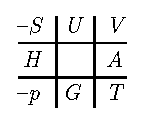
\includegraphics[scale=1.2]{thermo_square.eps}
    \end{framed}


$T$, $p$, and $\mu_{i}$ are intensive quantities, which do not depend on system size (same as density).\\[1ex]
$U$, $S$, $V$, and $n_{i}$ are extensive quantities, which grow linearly with system size (same as mass).\\[1ex]
From this and \eqn{eq:thermo-fundamental},
\begin{align}
    & U = T S - p V + \sum_{i} \mu_{i} n_{i} \\
    & S \dd{T} - V \dd{p} + \sum_{i} n_{i} \dd{\mu}_{i} = 0 
    & & \text{($T$, $p$, and $\mu_i$ are not mutually independent)
    \hspace*{0.1\columnwidth}} \label{eq:gibbs-duhem}
\end{align}

\subsection{Chemical equilibrium}

Partial pressures:
\begin{align}
    p_i & = \chi_{i} p & &
        \text{partial pressure of species $i$; $p$ is total pressure} \\
    \chi_i & = n_i/n_{\mathrm{tot}} & &
        \text{molar fraction of species $i$; $n_i$ is corresponding molar amount}
\end{align}
For the ideal gas, partial pressure is equal to the pressure it would exert if all other gaseous species were removed from the container, which means that its partial pressure depends
\textbf{only} on its amount, temperature and volume, and not on the amount of any other gasses:
\begin{equation}
    p_i V = n_i R T
\end{equation}
For this reason, from \eqn{eq:gibbs-duhem} at constant temperature ($\dd{T} = 0$),
\begin{subequations}
    \begin{align}
        n_{i} \dd{\mu_i} & = V \dd{p_{i}} \\
        \mu_i & = \mu_i\std + R T \ln(\frac{p}{p\std}) \qquad
        (p\std = \SI{1}{bar} = \SI{e5}{Pa} \text{ is the standard pressure})
    \end{align}        
\end{subequations}
From this, for an ideal-gas equilibrium \ce{A_{(g)} <=> B_{(g)}}
\begin{align}
    \DrG & = \DrG\std + R T \ln(\frac{p_{\rm B}/p\std}{p_{\rm A}/p\std}\!)
    = \DrG\std + R T \ln(Q)\\
    \DrG\std & = \mu_{\rm B}\std - \mu_{\rm A}\std = -R T \ln(\frac{p_{\rm B}/p\std}{p_{\rm A}/p\std}\!)_{\! \rm eq} = - R T \ln(K_{\rm eq})
    \label{eq:gibbs-keq}
\end{align}
where $Q$ is the reaction quotient. At equilibrium, $\DrG = 0$ and the quotient is equal to the equilibrium constant $K_{\rm eq}$. For 
general stoichiometry \ce{$\sum_{A} \nu_A$ A_{(g)} <=> $\sum_{B} \nu_B$ B_{(g)}},
\begin{equation}
    Q = \ln(
        \frac{\prod_{B} \qty(p_{\rm B} / p\std)^{\nu_B}}{
              \prod_{A} \qty(p_{\rm A} / p\std)^{\nu_A}
        }
    )
\end{equation}
In solution, $p/p\std$ is replaced with the activity $a$.
\begin{equation}
    a = \begin{cases}
        1 \text{ for a pure solid, liquid, or for the solvent} \\
        [\mkern14mu ]\text{ concentration in \SI{}{mol/dm^{-3}} for dilute solutes}
    \end{cases}
\end{equation}
For a dissolving solid \ce{AB_{(s)} <=> A^{+}_{(aq)} + B^{-}_{(aq)}} the equilibrium constant is
\begin{equation}
    K_{\rm sp} = [{\rm A}]_{\rm eq}[{\rm B}]_{\rm eq}
    \qquad \text{[solubility product]}.
\end{equation}

Van't Hoff isotherm:
\begin{align}
\qty(\pdv{G}{T})_{\!p,n_i} \!\! & = -S & &
\text{[from \eqn{eq:gibbs-master}]} \\
\qty(\pdv{(G/T)}{T})_{\!p,n_i} \!\! & =
\frac{1}{T} \qty(\pdv{G}{T})_{\!p,n_i} \!\! - \ 
\frac{G}{T^2} = -\frac{S}{T} - \frac{H - TS}{T^2} = -\frac{H}{T^2}
\end{align}
Also works if we replace the Gibbs energy with energy difference:
\begin{align}
    \qty(\pdv{(\DrG\std/T)}{T})_{\!p,n_i} \!\! & = 
    -\frac{\DrH\std}{T^2} & & \text{[generally true]} \\
    \qty(\pdv{\ln K_{\rm eq}}{T})_{\!p,n_i} \!\! & = 
    \frac{\DrH\std}{R T^2} & & \text{[from \eqn{eq:gibbs-keq}]} \\
    \ln(\frac{K_{\rm eq}(T_2)}{K_{\rm eq}(T_1)}) & = 
    -\frac{\DrH}{R} \qty(\frac{1}{T_2} - \frac{1}{T_1}) & &
    \text{[assuming that $\DrH\std$ does not depend on $T$]}
\end{align}

Electrochemical equilibria:
\begin{align}
    \mathcal{E} & = -\frac{\DrG\std}{\nu F} - \frac{R T}{\nu F} \ln Q = \mathcal{E}\std - \frac{R T}{\nu F} \ln Q \qquad \text{Nernst equation}\\
    \mathcal{E}\std  & = -\frac{\DrG\std}{\nu F} = \frac{R T}{\nu F} \ln K
\end{align}
where $\nu$ is the stoichiometric coefficient of the electrons in the cell half-reactions, $F = \SI{96485}{\ampere.\second / \mole}$ and $\mathcal{E}$ is the electromotive force (EMF) with units of \SI{}{\volt}.

Heat capacities:
\begin{align}
    C_{V} & = \qty(\pdv{U}{T})_{V} & & \text{constant-volume} \\
    C_{p} & = \qty(\pdv{H}{T})_{p} & & \text{constant-pressure} \\
    C_{p} & = C_{V} + n R & & \text{for the ideal gas
    \hspace*{0.45\columnwidth}}
\end{align}
For a gas of non-interacting rigid (non-vibrating) molecules

\begin{center}
\begin{tabularx}{0.675\textwidth}{|C|C|C|C|}
    \hline
     & \textbf{monoatomic} & \textbf{linear} & \textbf{non-linear} \\
    \hline
    \rule[-1.25em]{0pt}{3.5em}$\bm{C_{V}}$ & 
        $\displaystyle \frac{3}{2} n R$ &
        $\displaystyle \frac{5}{2} n R$ & 
        $\displaystyle 3 n R$ \\
    \hline
\end{tabularx}
\end{center}
If the molecules are vibrating, add an extra $n R$ for every ``active'' normal mode.

Kirchhoff's law (second equality assumes constant $C_p$)
\begin{align}
    H(T_2) & = H(T_1) + \int_{T_{1}}^{T_{2}} C_{p} \dd{T} = H(T_1) + C_{p} (T_2 - T_1)  & & \\
    S(T_2) & = S(T_1) + \int_{T_{1}}^{T_{2}} C_{p} \frac{\dd{T}}{T} = 
    S(T_1) + C_{p} \ln(\frac{T_2}{T_1})
\end{align}
The above is valid for heating of a single phase. If a phase transition occurs at temperature $T_{\rm tr}$ and with enthalpy $\Delta_{\rm tr} H$ 
then
\begin{align}
    H(T_2) & = H(T_1) + \int_{T_{1}}^{T_{\rm tr}} C_{p} \dd{T} + \Delta_{\rm tr} H + \int_{T_{\rm tr}}^{T_{2}} C_{p} \dd{T} \\
    S(T_2) & = S(T_1) + \int_{T_{1}}^{T_{\rm tr}} C_{p} \frac{\dd{T}}{T} + \frac{\Delta_{\rm tr} H}{T_{\rm tr}} + \int_{T_{\rm tr}}^{T_{2}} C_{p} \frac{\dd{T}}{T} 
\end{align}

Consider \eqn{eq:gibbs-duhem} for a single species in phase $\alpha$ (e.g., liquid) and phase $\beta$ (e.g., gas). 
\begin{align}
    \dd{\mu_{\alpha}} & = V_{\alpha, {\rm m}} \dd{p} - S_{\alpha, {\rm m}} \dd{T} \qquad \qquad
    \dd{\mu_{\beta}} = V_{\beta, {\rm m}} \dd{p} - S_{\beta, {\rm m}} \dd{T} 
\end{align}
where $V_{\alpha, {\rm m}}$ is the \emph{molar} volume of phase $\alpha$, 
$S_{\alpha, {\rm m}}$ is the \emph{molar} entropy of phase $\alpha$, etc. 
At equilibrium, $\mu_{\alpha} = \mu_{\beta}$, so that
$ \dd{\mu}_{\alpha} =  \dd{\mu}_{\beta}$ and along the phase boundary
\begin{gather}
    V_{\alpha, {\rm m}} \dd{p} - S_{\alpha, {\rm m}} \dd{T} = 
    V_{\beta, {\rm m}} \dd{p} - S_{\beta, {\rm m}} \dd{T} \\
    \shortintertext{or}
    \dv{p}{T} = \frac{\Delta_{\rm tr} S_{m}}{\Delta_{\rm tr} V_{m}}
    = \frac{\Delta_{\rm tr} H_{m}}{T \Delta_{\rm tr} V_{m}}
    \qquad \qquad \text{Clapeyron equation}
\end{gather}
For a liquid-to-gas transition (vaporisation) or solid-to-gas (sublimation), the change in volume is essentially equal to the volume of gas formed. Asuming ideality,
\begin{align}
    \Delta_{\rm tr} V_{m} & = \frac{R T}{p} \quad \Rightarrow \quad
    \dv{p}{T} = \frac{\Delta_{\rm tr} H_{m}}{R T^2 / p}  \quad \Rightarrow \quad
    \dv{\ln p}{T}  = \frac{\Delta_{\rm tr} H_{m}}{R T^2} \qquad 
    \text{(Clausius--Clapeyron)}
\end{align}

\subsection{pH calculation}

For \ce{H2O_{(l)} <=> H^{+}_{(aq)} + OH^{-}_{(aq)} }, the equilibrium constant
\begin{equation}
    \Kw = [\ce{H+}][\ce{OH-}] = \num{e-14}
\end{equation}
For a monoprotic acid \ce{HA_{(aq)} <=> H^{+}_{(aq)} + A^{-}_{(aq)}},
\begin{equation}
    \Ka = \frac{[\ce{H+}][\ce{A-}]}{[\ce{HA}]}
\end{equation}
We define
\begin{equation}
    \pH = -\log_{10} [\ce{H+}], \qquad
    \pKa = -\log_{10} \Ka
\end{equation}

For a monoprotic acid with total concentration $\ca$:
\renewcommand{\arraystretch}{1.5}
\begin{center}
    \begin{tabularx}{0.675\textwidth}{|c|c|C|}
        \hline
        $\pKa$ & $ \ca / M $ & [H\textsuperscript{+}] \\
        \hline
        $ {} < 0$ & $ {} > \num{e-6}$ & $\ca$ \\
        $ {} < 0$ & $ {} < \num{e-6}$ & $\frac{\ca}{2} + \sqrt{\qty(\frac{\ca}{2})^2 + \Kw}$ \\
        $0 \ldots 8$ & $ {} > \num{e-6} $ & 
        $ -\frac{\Ka}{2} + \sqrt{\qty(
            \frac{\Ka}{2}
        )^2 + \Ka \ca} $ \\
        ${} > 8$ & any & $\sqrt{\Ka \ca + \Kw}$ \\
        \hline
    \end{tabularx}
    \end{center}

Henderson--Hasselbalch equation:
\begin{equation}
    \pH = \pKa + \log_{10} \qty( \frac{[\ce{A-}]}{[\ce{HA}]} )
\end{equation}

\section{Kinetics}

\subsection{Enzyme kinetics}

\begin{reactions*}
    E + S  &<=>[\kn{1}][\kn{-1}] ES ->[\kn{2}] E + P
\end{reactions*}
E is the enzyme, S is the substrate, ES is the enzyme--substrate complex, and P is the product.
\begin{equation}
    \label{eq:MM-rate}
    \text{rate} = -\dv{[\ch{ES}]}{t} = k_2 [\ch{ES}]
\end{equation}

\paragraph{Pre-equilibrium assumption}

\begin{align}
    \frac{[\ch{ES}]}{[\ch{E}][\ch{S}]} = \frac{k_{1}}{k_{-1}} \quad & \Rightarrow \quad 
    [\ch{ES}] = \frac{k_{1}}{k_{-1}} [\ch{E}][\ch{S}]
    \label{eq:preeq-ES}
     \\
    [\ch{E}]_0 =  [\ch{E}] + [\ch{ES}] \quad & \Rightarrow \quad [\ch{E}] = [\ch{E}]_0 - [\ch{ES}] \\
    [\ch{ES}] = \frac{k_{1}}{k_{-1}} ([\ch{E}]_0 - [\ch{ES}]) [\ch{S}] 
    \quad & \Rightarrow \quad 
    [\ch{ES}] = \frac{\frac{k_1}{k_{-1}} [\ch{E}]_0 [\ch{S}]}{1 + \frac{k_1}{k_{-1}} [\ch{S}]}
    \label{eq:preeq-ES-final}
\end{align}
Putting \eqs{eq:MM-rate}{eq:preeq-ES-final} together,
\begin{gather}
    \text{rate} = \frac{v_{\text{max}} [\ch{S}]}{K_{\text{M}} + [\ch{S}]} \qquad
    \qty( v_{\text{max}} = k_2 [E]_{0} \qqtext{and}
    K_{\text{M}} = \frac{k_{-1}}{k_{1}} ) \label{eq:MM-rate-final}
\end{gather}

\paragraph{Steady-state assumption}

\begin{align}
\dv{[\ch{ES}]}{t} = k_1 [\ch{E}][\ch{S}] - k_{-1} [\ch{ES}] - k_{2} [\ch{ES}] = 0
\quad \Rightarrow \quad [\ch{ES}] = \frac{k_{1}}{k_{-1} + k_{2}} [\ch{E}] [\ch{S}]
\end{align}
The only change compared to the derivation using the pre-equilibrium assumption is that 
$\frac{k_1}{k_{-1}}$ in Eqs.~\eqref{eq:preeq-ES}--\eqref{eq:preeq-ES-final} is replaced with
$\frac{k_{1}}{k_{-1} + k_{2}}$, so that the rate still has the form in \eqn{eq:MM-rate}, except now $ K_{\text{M}} = \frac{k_{-1} + k_2}{k_{1}} $.

\subsubsection{Competitive inhibition}

\hspace*{2em}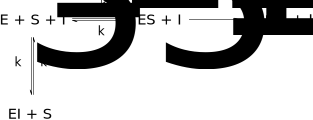
\includegraphics{competitive_inhibition.eps}\\

For the derivation, we will use the pre-equilibrium assumption. Let's define
\begin{equation}
    K_{\text{M}} = \frac{k_{-1}}{k_{1}} \qqtext{and} K_{\text{I}} = \frac{k_{-3}}{k_{3}} 
\end{equation}
Then
\begin{align}
    K_{\text{I}} = \frac{[\ch{E}][\ch{I}]}{[\ch{EI}]} \quad & \Rightarrow \quad
    [\ch{EI}] = \frac{[\ch{E}][\ch{I}]}{K_{\text{I}}} \\
    [\ch{E}]_0 =  [\ch{E}] + [\ch{ES}] + \underbrace{[\ch{EI}]}_{\mathclap{[\ch{E}][\ch{I}] / K_{\text{I}}}} \quad & \Rightarrow \quad [\ch{E}] = \frac{[\ch{E}]_0 - [\ch{ES}]}{1 + [\ch{I}] / K_{\text{I}}} \\ 
    K_{\text{M}} = \frac{[\ch{E}][\ch{S}]}{[\ch{ES}]} \quad & \Rightarrow \quad
    [\ch{ES}] = \frac{[\ch{E}][\ch{S}]}{K_{\text{M}}} = \frac{1}{K_{\text{M}}} 
    \qty(\frac{[\ch{E}]_0 - [\ch{ES}]}{1 + [\ch{I}] / K_{\text{I}}}) [\ch{S}]
\end{align}
Solving for $[\ch{ES}]$ we get
\begin{equation}
    \text{rate} = k_2 [\ch{ES}] = \frac{v_{\text{max}} [\ch{S}]}{K_{\text{M,eff}} + [\ch{S}]} 
\end{equation}
where $v_{\text{max}}$ is the same as in the uninhibited case, but
\begin{equation}
    K_{\text{M,eff}} = K_{\text{M}} \qty(1 + \frac{[\ch{I}]}{K_{\text{I}}}) > K_{\text{M}}
\end{equation}

\subsubsection{Uncompetitive inhibition}

\hspace*{2em}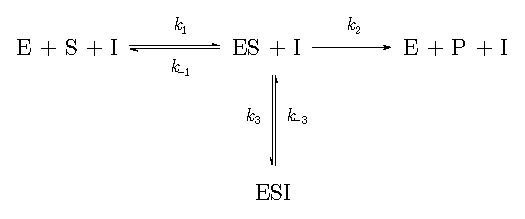
\includegraphics{uncompetitive_inhibition.eps}\\

$K_{\text{M}}$ and $K_{\text{I}} $ are defined as before but the pre-equilibrium approximation looks different:
\begin{align}
    K_{\text{I}} = \frac{[\ch{ES}][\ch{I}]}{[\ch{ESI}]} \quad & \Rightarrow \quad
    [\ch{ESI}] = \frac{[\ch{ES}][\ch{I}]}{K_{\text{I}}} \\
    [\ch{E}]_0 =  [\ch{E}] + [\ch{ES}] + \underbrace{[\ch{ESI}]}_{\mathclap{[\ch{ES}][\ch{I}] / K_{\text{I}}}} \quad & \Rightarrow \quad [\ch{E}] = [\ch{E}]_0 - [\ch{ES}]\qty(1 + [\ch{I}] / K_{\text{I}}) \\ 
    K_{\text{M}} = \frac{[\ch{E}][\ch{S}]}{[\ch{ES}]} \quad & \Rightarrow \quad
    [\ch{ES}] = \frac{[\ch{E}][\ch{S}]}{K_{\text{M}}} = \frac{1}{K_{\text{M}}} 
    \qty\Big( [\ch{E}]_0 - [\ch{ES}]\qty(1 + [\ch{I}] / K_{\text{I}})  ) [\ch{S}]
\end{align}
Solving for $[\ch{ES}]$ we get
\begin{equation}
    \text{rate} = k_2 [\ch{ES}] = \frac{v_{\text{max}} [\ch{S}]}{K_{\text{M}} + \qty(1 + \frac{[\ch{I}]}{K_{\text{I}}})[\ch{S}]} = 
    \frac{v_{\text{max,eff}} [\ch{S}]}{K_{\text{M,eff}} + [\ch{S}]}
\end{equation}
where
\begin{equation}
    v_{\text{max,eff}} = \frac{
        v_{\text{max}}
    }{
        1 + \frac{[\ch{I}]}{K_{\text{I}}}
    } \qqtext{and} 
    K_{\text{M,eff}} = \frac{
        K_{\text{M}}
    }{
        1 + \frac{[\ch{I}]}{K_{\text{I}}}
    }
\end{equation}
i.e., both the effective maximum rate and the effective Michaelis constant are reduced compared to the uninhibited case, and the reduction is by the same factor.


\subsubsection{Noncompetitive inhibition}

\hspace*{2em}\includegraphics{noncompetitive_inhibition.eps}\\

\begin{align}
    K_{\text{I}} & = \frac{[\ch{ES}][\ch{I}]}{[\ch{ESI}]} \ \Rightarrow \
    [\ch{ESI}] = \frac{[\ch{ES}][\ch{I}]}{K_{\text{I}}} \qqtext{and}
    K_{\text{I}} = \frac{[\ch{E}][\ch{I}]}{[\ch{EI}]} \ \Rightarrow \
    [\ch{EI}] = \frac{[\ch{E}][\ch{I}]}{K_{\text{I}}} \\
    [\ch{E}]_0 & =  [\ch{E}] + [\ch{ES}] 
        \ + \ \underbrace{[\ch{EI}]}_{\mathclap{[\ch{E}][\ch{I}] / K_{\text{I}}}}
        \ + \ \underbrace{[\ch{ESI}]}_{\mathclap{[\ch{ES}][\ch{I}] / K_{\text{I}}}}
        \ \Rightarrow \
        [\ch{E}] = \frac{[\ch{E}]_0 - [\ch{ES}]\qty(1 + [\ch{I}] / K_{\text{I}})}{1 + [\ch{I}] / K_{\text{I}}} = \frac{[\ch{E}]_0}{1 + [\ch{I}] / K_{\text{I}}} - [\ch{ES}] \\
    K_{\text{M}} & = \frac{[\ch{E}][\ch{S}]}{[\ch{ES}]} \ \Rightarrow \
        [\ch{ES}] = \frac{[\ch{E}][\ch{S}]}{K_{\text{M}}} = \frac{1}{K_{\text{M}}} 
        \qty\Big( \frac{[\ch{E}]_0}{1 + [\ch{I}] / K_{\text{I}}} - [\ch{ES}]  ) [\ch{S}]   
\end{align}
Solving for $[\ch{ES}]$,
\begin{equation}
    \text{rate} = k_2 [\ch{ES}] = \frac{v_{\text{max,eff}} [\ch{S}]}{K_{\text{M}} + [\ch{S}]}
\end{equation}
where
\begin{equation}
    v_{\text{max,eff}} = \frac{
        v_{\text{max}}
    }{
        1 + \frac{[\ch{I}]}{K_{\text{I}}}
    }
\end{equation}
and $K_{\text{M}}$ is unchanged from the uninhibited case.

\end{document}